\documentclass{article}

\usepackage{graphicx}
\usepackage{tikz}
\usepackage{tikzsymbols}
\usetikzlibrary{calc,patterns,shapes.geometric}
\pagestyle{empty}
\usepackage[margin=0pt]{geometry}
\geometry{papersize={14in,12in}}

\def\centerarc[#1](#2)(#3:#4:#5){\draw[#1] ($(#2)+({#5*cos(#3)},{#5*sin(#3)})$) arc (#3:#4:#5);}

\begin{document}
	\begin{figure}
		\centering
		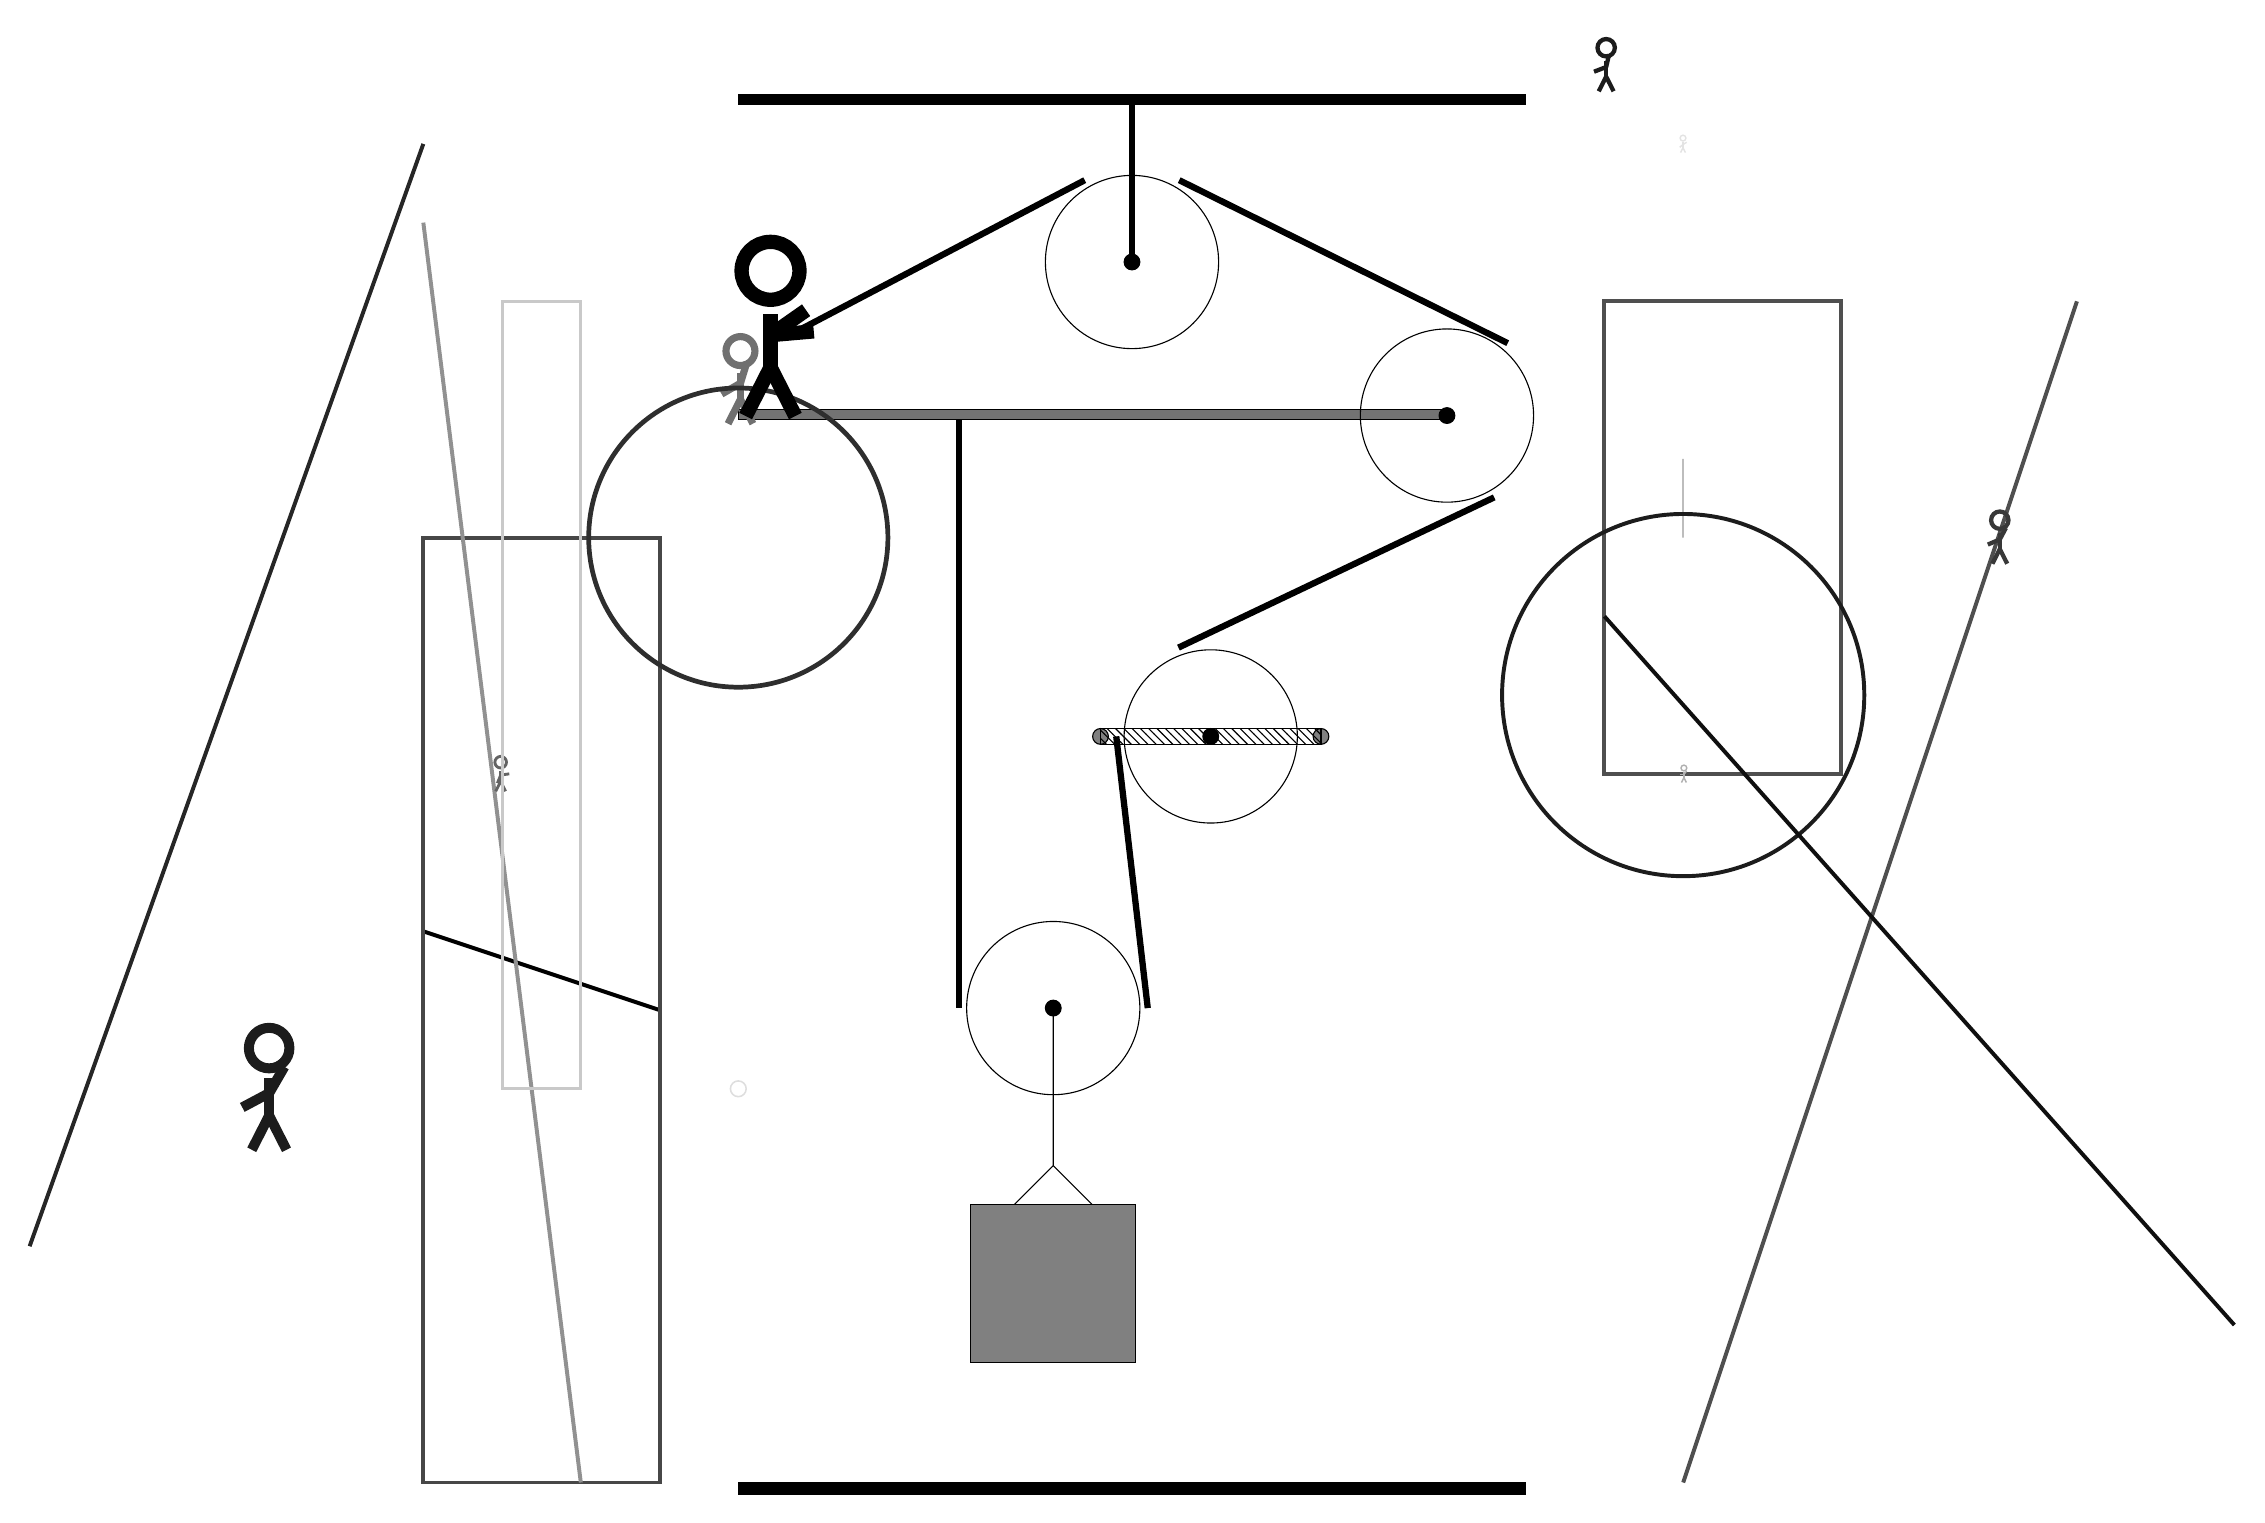
\begin{tikzpicture}
			%%%%% START %%%%%
			
			\draw[fill=black] (-2, 15.5) rectangle (8, 15.625);
			
			\draw[fill=black!55] (-2, 11.5) rectangle (7, 11.625);
			
			\draw (2, 4.025) circle (1.1);
			\draw[fill=black] (2, 4.025) circle (0.1);
			
			\draw (7, 11.55) circle (1.1);
			\draw[fill=black] (7, 11.55) circle (0.1);
			
			\draw[line width=0.5mm, color=black!100](-3, 4) -- (-6, 5);
			
			\draw[line width=0.5mm, color=black!72] (-3, 10) rectangle (-6, -2);
			\node[line width=0.2mm, color=black!89] at (9, 16) {\Strichmaxerl[3][21][77]};
			\draw [line width=0.2mm, color=black!13](-2, 3) circle (0.1);
			\draw[line width=0.5mm, color=black!69] (9, 13) rectangle (12, 7);
			\node[line width=0.7mm, color=black!56] at (-2, 12) {\Strichmaxerl[5][30][73]};
			\draw [line width=0.6mm, color=black!82](-2, 10) circle (1.9);
			\draw[line width=0.5mm, color=black!69](10, -2) -- (15, 13);
			\draw[line width=0.5mm, color=black!43](-6, 14) -- (-4, -2);
			\node[line width=0.7mm, color=black!31] at (10, 7) {\Strichmaxerl[1][0][52]};
			\draw[line width=0.3mm, color=black!26] (10, 11) rectangle (10, 10);
			\node[line width=0.4mm, color=black!61] at (-5, 7) {\Strichmaxerl[2][68][8]};
			\draw[line width=0.5mm, color=black!85](-6, 15) -- (-11, 1);
			
			\node[line width=0.7mm, color=black!11] at (10, 15) {\Strichmaxerl[1][40][32]};
			\draw [line width=0.5mm, color=black!89](10, 8) circle (2.3);
			\draw[line width=0.4mm, color=black!21] (-4, 13) rectangle (-5, 3);
			\node[line width=0.7mm, color=black!78] at (14, 10) {\Strichmaxerl[3][23][62]};
			
			\draw[line width=0.5mm, color=black!94](9, 9) -- (17, 0);
			\node[line width=0.3mm, color=black!89] at (-8, 3) {\Strichmaxerl[7][28][60]};
			
			\draw[fill=white](4, 7.475) circle (1.1);
			\draw[fill=black] (4, 7.475) circle (0.1);
			\draw[fill=black!50] (2.6, 7.475) circle (0.1);
			\draw[fill=black!50] (5.4, 7.475) circle (0.1);
			\draw[pattern=north west lines, pattern color=black] (2.6, 7.575) rectangle (5.4, 7.375);
			
			\draw (3, 13.5) circle (1.1);
			\draw[fill=black] (3, 13.5) circle (0.1);
			\draw[line width=0.8mm] (3, 13.5) -- (3, 15.5);
			
			\draw (2, 4.025) -- (2, 2.025) -- (1.5, 1.525) -- (2.5, 1.525) -- (2, 2.025);
			\draw[fill=black!50] (0.95, 1.525) rectangle (3.05, -0.475);
			
			\draw[line width=0.8mm] (0.8, 11.5) -- (0.8, 4.025);
			\centerarc[line width=0.8mm](2, 4.025)(180:360:1.2000000000000002);
			\draw[line width=0.8mm](3.2, 4.025) -- (2.8, 7.475);
			\centerarc[line width=0.8mm](4, 7.475)(110:180:1.2000000000000002);
			\draw[line width=0.8mm](3.5896, 8.6026) -- (7.6, 10.5108);
			\centerarc[line width=0.8mm](7, 11.55)(-60:50:1.2000000000000002);
			\draw[line width=0.8mm](7.7714, 12.4692) -- (3.6, 14.5392);
			\centerarc[line width=0.8mm](3, 13.5)(60:120:1.2000000000000002);
			\draw[line width=0.8mm](2.4, 14.5392) -- (-1.2, 12.65);
			
			\node at (-1.5, 12.65) {\Strichmaxerl[10][-175][35]};
			
			\draw[fill=black] (-2, -2) rectangle (8, -2.15);
			
			%%%%% END %%%%%
		\end{tikzpicture}
	\end{figure}	
\end{document}